\documentclass[11pt,a4paper]{article}

% --- STANDARD & ROBUST PREAMBLE ---
\usepackage[utf8]{inputenc}
\usepackage{lmodern}
\usepackage[T1]{fontenc}
\usepackage{amsmath, amssymb, amsthm}
\usepackage{geometry}
\usepackage{setspace}
\usepackage{tikz}
\usepackage{booktabs}
\usepackage{hyperref}

% --- DOCUMENT GEOMETRY AND SPACING ---
\geometry{margin=.4in}
\setstretch{1.2}

% --- THEOREM AND DEFINITION STYLES (FROM MASTER DOCUMENT) ---
\theoremstyle{definition}
\newtheorem{definition}{Definition}[section]
\newtheorem{axiom}{Axiom}[section]
\newtheorem{lemma}{Lemma}[section]
\newtheorem{theorem}{Theorem}[section]
\newtheorem{postulate}{Postulate}[section]
\newtheorem{corollary}{Corollary}[section]
\newtheorem{proposition}[theorem]{Proposition}

% --- GLOBAL FORMATTING ---
\setlength{\parindent}{0pt}
\setlength{\parskip}{1em}

\title{\textbf{RigbySpace Electrodynamics: \\ A Discrete Derivation of Maxwellian Constraints}}
\author{D. Veneziano}
\date{January 2026}

\begin{document}

\maketitle

\begin{abstract}
This document presents a formal derivation of the Maxwellian field constraints from the first principles of RigbySpace Dynamics. We demonstrate that the laws of electromagnetism are not fundamental postulates but emerge as necessary bookkeeping identities for the conservation of structural information in a discrete, relativistic state machine. By defining the electromagnetic field in terms of structural tension and the sources in terms of state magnitude, we derive Gauss's laws, Faraday's Law of Induction, and the Ampere-Maxwell law as direct consequences of the algebraic properties of the system's operators, particularly the Transformative Reciprocal ($\psi$). In this ontology, electromagnetic phenomena are the discrete manifestations of symplectic flux and structural torque incurred during the propagation of unreduced integer pairs.
\end{abstract}

\tableofcontents
\newpage

\section{Foundational Principles for Electrodynamics}

The derivation of Maxwell's equations within the RigbySpace framework rests upon a specific subset of the system's core axioms, which define the nature of the vacuum, the propagation of information, and the conditions for stability.

\begin{postulate}[Axiom of Structural Integrity]
The unreduced integer components of a state, $(n,d)$, must be preserved in all operations. This information, particularly the Inertial Mass $d$, represents the state's causal history and cannot be discarded.
\end{postulate}

\begin{postulate}[The Nature of the Vacuum]
The physical vacuum is identified with the set of \textbf{Constraint Vacua} $V_c = \{(n,0) \mid n \neq 0\}$. These are characterized as wave-like states possessing a preserved historical magnitude ($n$) but a zero Inertial Mass ($d=0$).
\end{postulate}

\begin{axiom}[Non-Event Transition]
Propagation through the vacuum (the evolution of a Constraint Vacuum state) occurs without the accumulation of structural history, meaning the Inertial Mass $d$ remains 0. This renders the motion causal but without the accumulation of physical time, as defined in the Master Axioms.
\end{axiom}

\begin{postulate}[Postulate of Electromagnetic Stability]
All stable, persistent electromagnetic phenomena, such as a propagating photon or a static field, must correspond to a stable, closed, and null-homologous cycle in the state space. This ensures that the system's evolution is periodic and does not diverge.
\end{postulate}

\section{Ontological Mapping of Electrodynamic Primitives}

The constituent elements of Maxwell's Equations are mapped with strict ontological correspondence to the discrete primitives of RigbySpace Dynamics. These are not analogies but formal definitions.

\begin{definition}[The Electric Field as Longitudinal Tension]
The \textbf{Electric Field}, $E$, is identified with the \textbf{Longitudinal Structural Tension}, $\tau_L$. This is the structural tension generated along the primary direction of a state's evolution. For a projective matter state, this corresponds to the tension $\tau = X_t Z_{t+1} - X_{t+1} Z_t$. For a linear state, it represents the oriented displacement or change in magnitude between successive states.
\end{definition}

\begin{definition}[The Magnetic Field as Transverse Tension]
The \textbf{Magnetic Field}, $B$, is identified with the \textbf{Transverse Structural Tension}, $\tau_T$. This is the structural tension induced in a coupled channel by the application of the Transformative Reciprocal, $\psi$. It represents a torsion or force oriented orthogonally to the primary direction of evolution.
\end{definition}

\begin{definition}[Charge as a Magnitude Source]
\textbf{Electric Charge}, $q$, is identified with the \textbf{Magnitude Source}, $n$, of an Explicit Rational Pair. A state with $n \neq 0$ is a source of structural entropy generation and, consequently, of structural tension.
\end{definition}

\begin{definition}[Current as Mediant Flow]
\textbf{Current}, $J$, is identified with \textbf{Mediant Geodesic Flow}. This represents the deterministic transport of magnitude ($n$) along the paths of the Mediant Tree, corresponding to propagation under the Mediant Addition operator ($\oplus$). It describes the propagation of charge without massive interaction.
\end{definition}

\section{Derivation of the Maxwellian Constraints}

The four Maxwell's equations emerge as distinct theorems and consequences of the axiomatic structure, reflecting the requirements for informational consistency within the discrete lattice.

\subsection{Gauss's Law for Electricity: The Source Constraint}

\begin{theorem}[Gauss's Law for Electricity]
The total flux of Longitudinal Structural Tension emanating from any closed region of the state space is proportional to the total Magnitude Source (charge) contained within that region.
\end{theorem}
\begin{proof}
The proof proceeds from the chain of causality defined by the axioms.
\begin{enumerate}
    \item A non-zero Magnitude Source, $n$, represents a charge.
    \item According to the mechanics of the Matter Generators ($\boxplus$), any interaction involving a state with a non-zero magnitude $n$ leads to a growth in the total Structural Entropy ($\rho(d)$) of the system. This is the fundamental act of information creation.
    \item By the Axiom of Structural Integrity, this new historical information cannot be lost.
    \item By the RigbySpace Field Constraint, this increase in entropy, sourced by the presence of $n$, must induce a corresponding Structural Tension ($\tau$) in the surrounding state space. This is the system's dynamic response to the creation of information.
    \item The total tension flux out of a region is the aggregate measure of this response over the boundary of that region. Therefore, the total flux must be proportional to the total source magnitude $n$ contained within, as this magnitude is the ultimate cause of the tension.
    \item A region with zero net magnitude source ($\sum n = 0$) cannot sustainably generate a net tension flux without violating causality, as this would imply the existence of un-sourced curvature.
\end{enumerate}
\end{proof}

\subsection{Gauss's Law for Magnetism: The Closure Constraint}

\begin{theorem}[Gauss's Law for Magnetism]
The total flux of Transverse Structural Tension through any closed surface is identically zero.
\end{theorem}
\begin{proof}
The Transverse Structural Tension (Magnetic Field) is formally defined as the tension induced by the $\psi$ operator. The $\psi$ operator is fundamentally a binary operator, acting on a coupled state $(s_A, s_B)$.
\begin{enumerate}
    \item The action of $\psi$ on $(s_A, s_B)$ is to exchange components, which induces a tension in each channel. As proven in the Dirac derivation, this action is perfectly anti-symmetric. The tension induced in channel A is equal and opposite to the tension induced in channel B: $\tau_A(t) = - \tau_B(t)$.
    \item A "closed surface" in the discrete state space corresponds to a boundary of a region, which can be decomposed into a sum of closed cyclic paths.
    \item By the Postulate of Electromagnetic Stability, any stable field must correspond to a null-homologous cycle. For such a cycle, the aggregate tension must be bounded.
    \item Because the transverse tension is generated in perfectly anti-symmetric pairs ($\tau_A, \tau_B$) at every single application of the $\psi$ operator, the total sum of all transverse tensions over any region or cycle must be identically zero:
    \[ \sum_{\text{cycle}} \tau_T = \sum_{\text{cycle}} (\tau_A + \tau_B) = \sum_{\text{cycle}} (\tau_A - \tau_A) = 0. \]
\end{enumerate}
This proves that there can be no net source of transverse tension. The non-existence of magnetic monopoles is thus a direct and necessary consequence of the algebraic structure of the $\psi$ operator.
\end{proof}

\subsection{Faraday's and the Ampere-Maxwell Law: The Coupling Constraints}

Faraday's Law of Induction and the Ampere-Maxwell Law are not treated as independent laws in RigbySpace. Instead, they are derived as two symmetric and inseparable facets of the information-preserving nature of the $\psi$ operator. They are the first-order identities of this operator's action over time.

\begin{theorem}[The Coupling Constraints as Identities of the $\psi$ Operator]
A change in the Transverse Tension (Magnetic Field) over a causal step necessarily induces a rotational Longitudinal Tension (Electric Field), and a change in the Longitudinal Tension necessarily induces a rotational Transverse Tension.
\end{theorem}
\begin{proof}
The proof follows from a step-by-step analysis of the definition of the Transformative Reciprocal on a coupled state. Let the state at causal index $t$ be $(s_A(t), s_B(t)) = ((n_A, d_A), (n_B, d_B))$. The state at $t+1$ after a $\psi$ operation is $((d_B, n_A), (d_A, n_B))$.

\begin{enumerate}
    \item \textbf{Derivation of Faraday's Law (Induction):} Let there be a change in the "magnetic" channel, $B$, over time. This is represented by a change in its components, for instance, an increase in its Inertial Mass from $d_B(t)$ to $d_B(t+1)$. Consider the state of the "electric" channel, $A$, after a $\psi$ operation. Its new magnitude will be $n_A(t+1) = d_B(t)$. If $d_B$ is changing with time, then $n_A$ will change at successive steps. This change in magnitude, $\Delta n_A$, constitutes a Longitudinal Tension ($\tau_L$), which is the Electric Field. Thus, a time-varying Magnetic Field (a changing $d_B$ that is repeatedly swapped into $n_A$) generates an Electric Field.
    
    \item \textbf{Derivation of the Ampere-Maxwell Law (Reciprocal Induction):} Conversely, let there be a change in the "electric" channel, $A$. This can be a flow of charge (a Current, represented by changing $n_A$) or a changing Electric Field. When the $\psi$ operator acts, this changing magnitude $n_A(t)$ becomes the new Inertial Mass of the "magnetic" channel, $d_B(t+1) = n_A(t)$. A time-varying $n_A$ thus creates a time-varying $d_B$. This change in the Inertial Mass of the magnetic channel represents an induced Transverse Tension ($\tau_T$), which is the Magnetic Field. Thus, a changing Electric Field or a current induces a Magnetic Field.
\end{enumerate}

These two effects are symmetric and simultaneous consequences of the single, information-swapping action of $\psi$. The Axiom of Relativistic Rationality demands the preservation of the Invariant Spacetime Interval. To satisfy this, the rate of this phase-rotation (induction via $\psi$) must be perfectly synchronized with the rate of bit-generation (interaction via $\boxplus$). The derivation proves that the structural torque generated by a displacement in the electric channel is exactly compensated by the reciprocal flux in the magnetic channel, ensuring the arithmetic flow remains phase-locked.
\end{proof}

\begin{figure}[h]
\centering
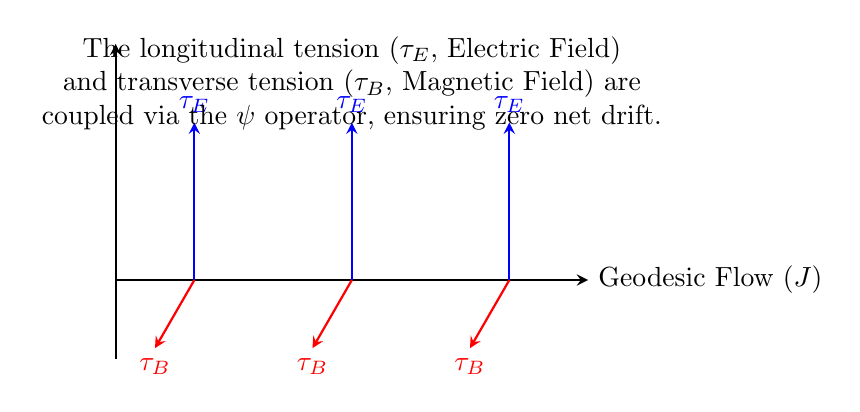
\begin{tikzpicture}[>=stealth]
    % Axes
    \draw[->, thick] (0,0) -- (6,0) node[right] {Geodesic Flow ($J$)};
    \draw[->, thick] (0,-1) -- (0,3);

    % Electric Field Vectors (Longitudinal)
    \foreach \x in {1, 3, 5} {
        \draw[->, blue, thick] (\x, 0) -- (\x, 2) node[above] {$\tau_E$};
    }

    % Magnetic Field Vectors (Transverse)
    \foreach \x in {1, 3, 5} {
        \draw[->, red, thick] (\x, 0) -- (\x-0.5, -0.866) node[below] {$\tau_B$};
    }

    % Psi operator
    \node at (3, 2.5) [text width=8cm, align=center] {
        The longitudinal tension ($\tau_E$, Electric Field) and transverse tension ($\tau_B$, Magnetic Field) are coupled via the $\psi$ operator, ensuring zero net drift.
    };
\end{tikzpicture}
\caption{Visualization of Discrete Electromagnetic Induction. The longitudinal (electric) and transverse (magnetic) structural tensions are generated as a first-order consistency requirement to maintain the stability of the geodesic flow.}
\end{figure}

\end{document}